La humanitat ha estat exposada a la radioactivitat des de l'inici dels temps, ja siga procedent de fonts extraterrestres o de la propia escorça terrestre. Des que Henry Becquerel va descobrir la radioactivitat en $1896$, s'ha desenvolupat molta tecnologia nuclear en diferents camps com ara la medicina, la investigació, la producció de energia, etc. Aquesta creació de fonts nuclears antropogèniques ha conduït a un excés de elements radioactius lliberats al medi ambient i, consegüentment, a un augment de la dosi radioactiva a què els essers humans ens veiem afectats. Aquest augment es pot observar a la Figura  \ref{fig:RadioactiveDosePopulation}, que mostra la distribució de la mitjana anual de la dosi radioactiva rebuda per la població mundial.

\begin{figure}[h]
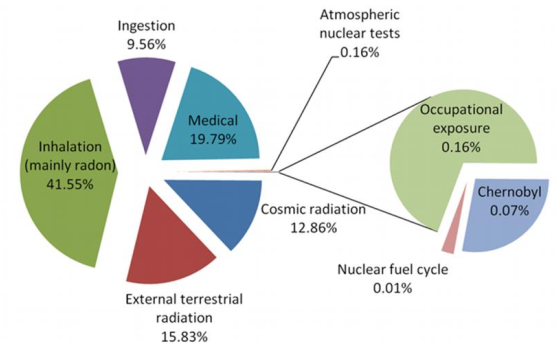
\includegraphics[scale=0.5]{12Summary/2Introduction/RadioactiveDosePopulation.png}
\centering
\caption{Mitjana anual de la dosi radioactiva rebuda per la població mundial~\cite{IAEA}\label{fig:RadioactiveDosePopulation}.}
\end{figure}

A causa d'aquest augment dels nivells de radioactivitat en el medi ambient és important fer un control per assegurar que aquest es troben per baix dels límits considerats segurs per a la població. A Espanya, aquest control el realitza el Consell de Seguritat Nuclear (CSN) \cite{CSN}, l'única autoritat a Espanya en matèria de seguretat nuclear i radioprotecció. Per realitzar aquesta tasca de control, el CSN disposa de diverses xarxes entre les quals se encontra la xarxa d'estacions de monitorització (REM per les sigles en castellà). En aquesta, al voltant de 20 laboratoris espanyols prenen mostres en diferents punts del país per caracteritzar, quantificar i controlar les concentracions de radioisòtops presents en el medi ambient.

Un dels radioisòtops habitualment medit en aquests tests es el triti, el tercer isòtop de l'hidrogen. Es tracta de un element amb una vida mitja de $T_{1/2} = 12.32$ anys que únicament es desintegra via $\beta^{-}$ emitint un electró i un neutrí a través del proces:
\begin{equation}
\ce{^{3}_{1}H} \longrightarrow \ce{^{3}_{2}He}  + \ce{e^-}  + \ce{\overline{\nu}_e}
\label{eq:DecaimentTriti}
\end{equation}

El nivell de triti en el medi ambient, excloent les fonts antropogèniques radioactives actuals, es troba entre $1$ y $4~\becquerel/\liter$, més gran que el esperat ($0.6-1.2~\becquerel/\liter$) a causa de les proves nuclears realitzades en el passat \cite{FranceTritiumEnvironment}. Aquest nivell augmenta fins a $10~\becquerel/\liter$ en els llocs al voltant de les centrals nuclears y fins a entre $20$ y $50~\becquerel/\liter$ al lloc on la central nuclear descarrega l'aigua empleada en la refrigeració del nucli \cite{FranceTritiumEnvironment}. Un exemple d'aquest augment el trobem als tests realitzats pel REM al voltant de la central nuclear de Cofrents, Valencia. En aquests tests el triti és mesurat en tres punts del riu Júcar assenyalats en la Figura \ref{fig:PuntsMesuraTritiCofrents}, els quals se encontren a $6~\kilo\meter$ abans de la central nuclear, $1~\kilo\meter$ després y $5~\kilo\meter$ després, respectivament representats per el punts P1, P2 i P3. Los mesures de triti en aquestes zones es veues respectivamente representades en les gràfiques de la Figura \ref{fig:MesuresSuperficialsCofrents}. En aquestes gràfiques el limit de detecció i la activitat mesurada per al triti es representen en punts blancs i verds respectivament. Com es pot comprobar, el nivell de triti augmenta just després de la central nuclear y, paulatinament es va reduint a causa de la dissolució del triti en l'aigua. És important remarcar que, encara que aquests nivells de triti si han aumentat a causa de la central nuclear, aquests mai han sobrepassat el límit permès. A Espanya, aquest limit és fixat per la directiva del consell EURATOM a $100~\becquerel/\liter$ per a l'aigua potable \cite{100BqL} mentres que el màxim nivell de triti mesurat des de l'any $2006$ únicament és de $32~\becquerel/\liter$.

Aquests nivells de triti també han sigut mesurats en altres dos punts de aigues subterrànies, uno situat $1~\kilo\meter$ abans de la central nuclear y l'altre situat $1~\kilo\meter$ després, representats pels punts S1 y S2 de la Figura \ref{fig:PuntsMesuraTritiCofrents}. En aquest cas, com és pot veure en les gràfiques de la Figura \ref{fig:MesuresSuperterraniesCofrents}, el nivell de triti no es veu afectat ja que la central nuclear únicament utilitza l'aigua del riu per a la refrigeració.

\begin{figure}[hbtp]
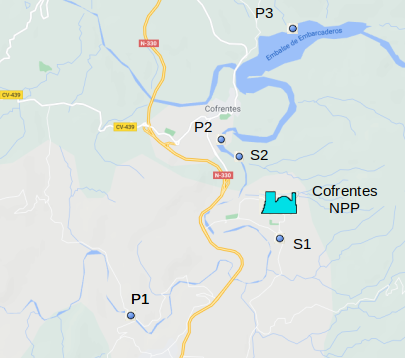
\includegraphics[scale=0.5]{12Summary/2Introduction/CofrentesMaps.png}
\centering
\caption{Punts de mesura de triti al voltant de la central nuclear de Cofrents.\label{fig:PuntsMesuraTritiCofrents}}
\end{figure}

\begin{figure}
\centering
    \begin{subfigure}[b]{0.7\textwidth}
    \centering
    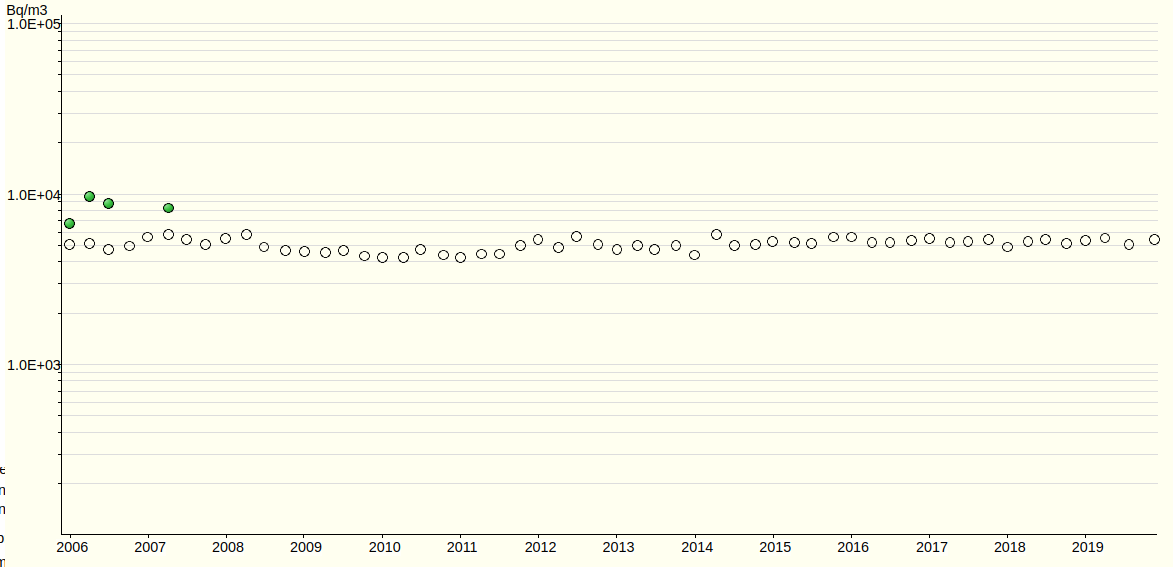
\includegraphics[width=\textwidth]{12Summary/2Introduction/6km_before.png}  
    \caption{\label{subfig:TritiumL6kB}}
    \end{subfigure}
    \hfill
    \begin{subfigure}[b]{0.7\textwidth}
    \centering
    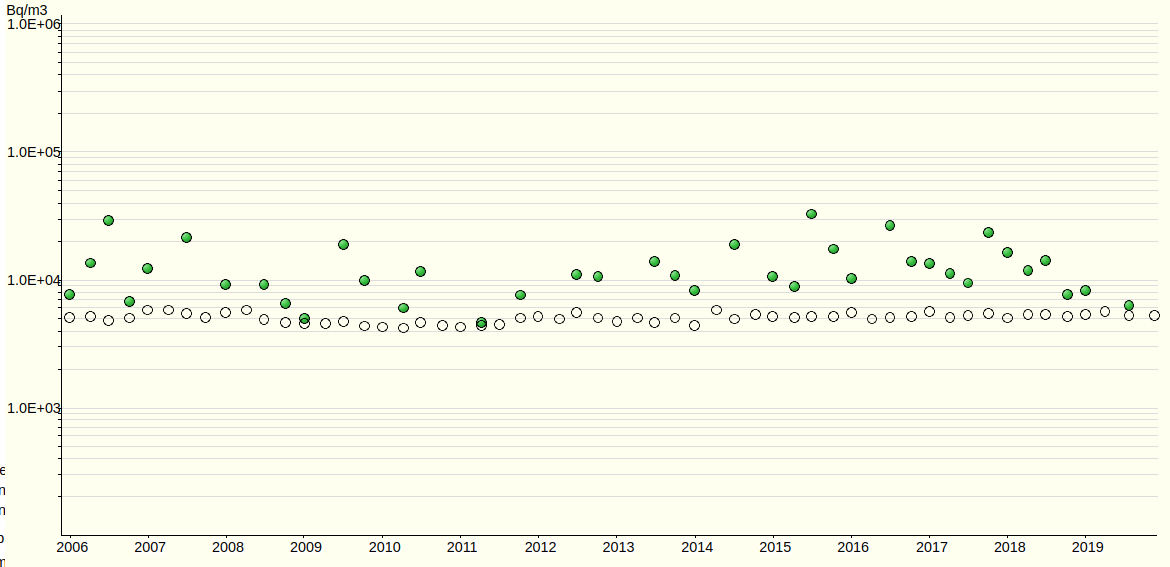
\includegraphics[width=\textwidth]{12Summary/2Introduction/1km_after.png}  
    \caption{\label{subfig:TritiumL1kA}}
    \end{subfigure}
    \hfill
    \begin{subfigure}[b]{0.7\textwidth}
    \centering
    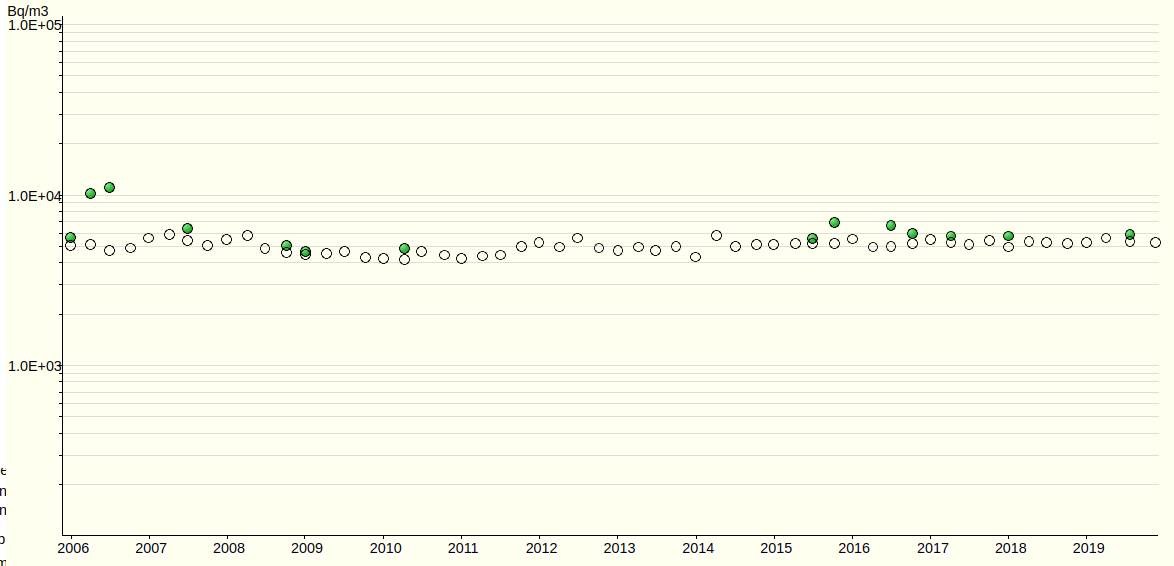
\includegraphics[width=\textwidth]{12Summary/2Introduction/5km_after.png}  
    \caption{\label{subfig:TritiumL5kA}}
    \end{subfigure}
 \caption{Nivell de activitat de triti in aigües superficials del riu Júcar des del gener de $2006$ fins al novembre de $2019$. (a) punt de mostra situat a $6~\kilo\meter$ de la central nuclear riu amunt. (b) $1~\kilo\meter$ riu avall. (c) $5~\kilo\meter$ riu avall. Els punts blancs y verds representen el límit de detecció y l'activitat mesurada respectivament. El màxim nivell de triti mesurat és al voltant de $32~\becquerel/\liter$.~\cite{REM}}
 \label{fig:MesuresSuperficialsCofrents}
\end{figure}

\begin{figure}
\centering
    \begin{subfigure}[b]{0.7\textwidth}
    \centering
    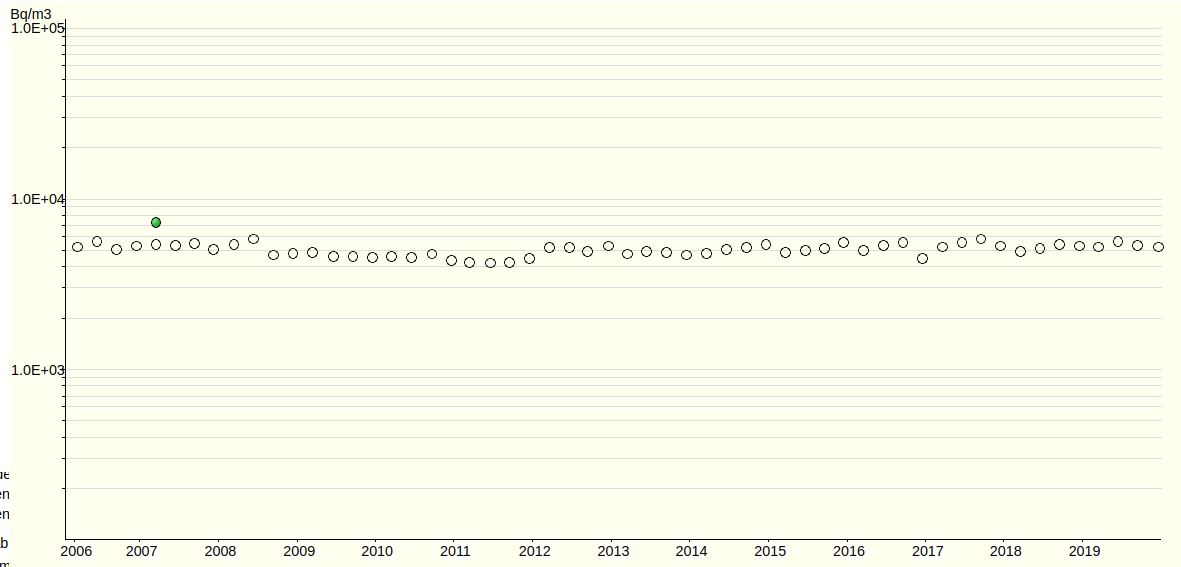
\includegraphics[width=\textwidth]{12Summary/2Introduction/Subterranea_before.png}  
    \caption{\label{subfig:TritiumLG1kB}}
    \end{subfigure}
    \hfill
    \begin{subfigure}[b]{0.7\textwidth}
    \centering
    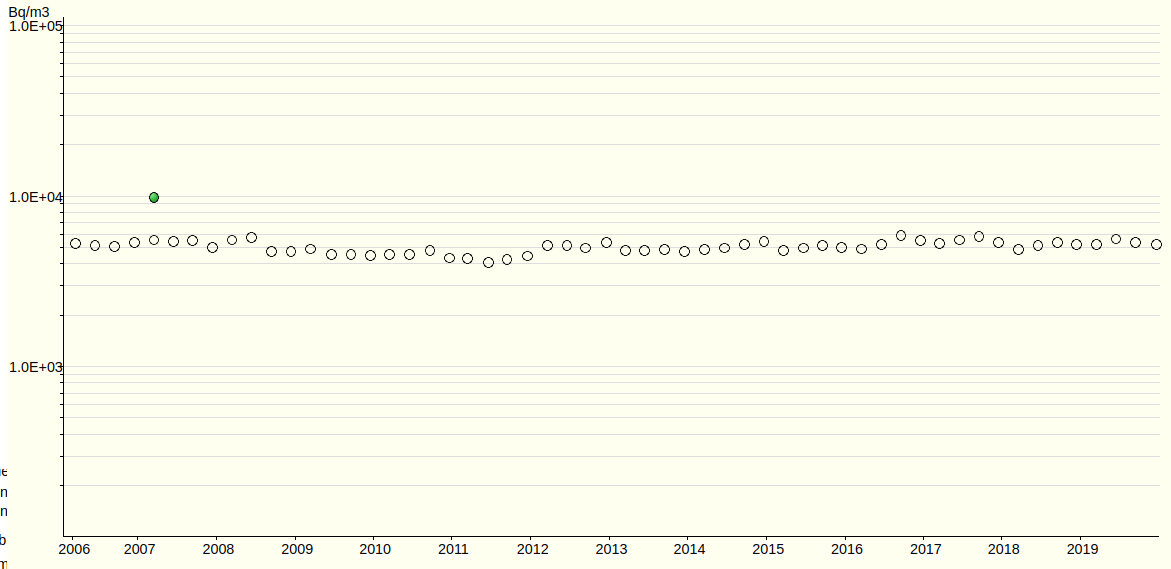
\includegraphics[width=\textwidth]{12Summary/2Introduction/Subterranea_1_km_later.png}  
    \caption{\label{subfig:TritiumLG1kA}}
    \end{subfigure}
 \caption{Nivell de l'activitat del triti en agües subterrànies al voltat de la central nuclear de Cofrents mesurats des del gener de $2006$ fins al novembre de $2019$~\cite{REM}. (a) $1~\kilo\meter$ de la central nuclear riu amunt. (b) $1~\kilo\meter$ de la central nuclear riu avall.~\cite{REM}}
 \label{fig:MesuresSuperterraniesCofrents}
\end{figure}

El triti és el radioisòtop amb una energia de desintegració meś baixa (una energia màxima de $Q_\beta=18.6~\keV$), raó per la qual presenta una baixa penetració en la pell. No obstant això, aqueste por arribar a ser altament perjudicial si s'introdueix en el cos, ja sigui ingerit o inhalat, ja que pot participar en reaccions químiques substituït al hidrogen i permaneixer fins a 50 díes \cite{EstimationTritiumDosiKangarooRats, TissueDistribution}, temps durant el qual estem rebent radiació. Es tracta d'un element radioactiu que afecta a la salut dels organismes vius si estan exposats a quantitats altes o de forma crònica, i poden arribar a causar mutacions de l'ADN, mort celular, pèrdua de la funcionalitat d'organs o desanvolupar tumors \cite{StraumeTritiumHazard}. A causa del perill que representa el triti per a la salut del éssers vius, molts països han creat lleis per regular l'alliberament de triti al medi ambient. Com ja s'ha comentat anteriorment, a Espanya, igual que A França i Alemania, aquest límit és fixat per la directiva del consell EURATOM a $100~\becquerel/\liter$ per a l'aigua potable. Aquest és un dels límits més restrictius entre els implantats als diferents països.

Les tècniques utilitzades hui en dia per a la mesura del triti, com pot ser el recompte de centelleigs líquids (LSC per les seues singles en anglès) o la mesura amb plastics de centelleig llegits per fotosensors, presenten l'inconvenient que o bé no son capaços de mesurar activitats tan baixes (mínima activitat detectable (MDA per les sigles en anglès) de milers de $~\becquerel/\liter$ en el millor dels casos) o bé necessiten molt de temps per a realitzar la mesura (més de dos dies), impossibilitant-los per ser empleats per a una monitorització del triti ambiental en temps quasi-real (menys de una hora).

Per superar aquest inconvenients es va proposar l'any $2016$ el projecte anomenat \textit{TRITIUM} (triti amb anglès), amb el títol "Diseny, construcció y manteniment de una estació automàtica per a la monitorització de baixos nivells d'activitat del triti en aigua". TRITIUM és una colaboració internacional formada per $6$ institucions procedents de $3$ països europeus, França, Portugal i Espanya.

L'objectiu d'aquest project és desenvolupar un monitor de nivells de triti que permeta obtenir mesures en temps quasi-real. Per a complir aquesta necessitat de temps quasi-real és imprescindible que el detector siga capaç de realitzar mesures ``in situ'', es a dir, al mateix lloc os es pren la mostra.

Com es veurà en la secció \ref{subsec:PrincipisDiseny}, la col·laboració TRITIUM aposta per un disseny del detector basat en milers de fibres de centelleig llegides per fotosensors. Aquestes fibres es posen directament en contacte amb la mostra a analitzar (aigua), les quals són capaces de detectar part dels decaïments radioactius del triti ocorreguts. A més, com es discutirà en la secció següent, s'han afegit alguns elements addicionals a aquest detector per tal de millorar la seua sensibilitat a la detecció del triti, com ara un sistema de rejecció del fons radioactiu o un sistema de purificació de l'aigua. L'objectiu final d'aquest serà instal·lar el monitor construït a la presa d'Arrocampo, a Extremadura, Espanya, al punt on l'aigua utilitzada per refrigerar el nucli de la central nuclear de Almaraz es alliberada al riu Tajo. L'aigua d'aquest riu és utilizada per espanyols y portuguesos, tant pel consum com pel regadiu, de manera que preservar-ne el correcte estat d'aquesta és un punt prioritari que afecta directament la salut de les persones. 